
% Created 2012-03-29 Thu 12:41
\documentclass[a4paper]{article}
\usepackage[utf8]{inputenc}
\usepackage[T1]{fontenc}
\usepackage{fixltx2e}
\usepackage{graphicx}
\usepackage{longtable}
\usepackage{float}
\usepackage{wrapfig}
\usepackage{soul}
\usepackage{textcomp}
\usepackage{latexsym}
\usepackage{amssymb}
\usepackage{hyperref}
\tolerance=1000
\usepackage{verbatim}
\setlength{\parindent}{0in}
\providecommand{\alert}[1]{\textbf{#1}}

\title{Letters analysis}
\author{Ivan Hanigan}
\date{\today}
\hypersetup{
  pdfkeywords={},
  pdfsubject={},
  pdfcreator={Emacs Org-mode version 7.8.03}}

\begin{document}

\maketitle

\setcounter{tocdepth}{3}
\tableofcontents
\vspace*{1cm}
\hrule

\section{Intro}
\clearpage
\section{First letter}
\begin{figure}[!h]
\centering
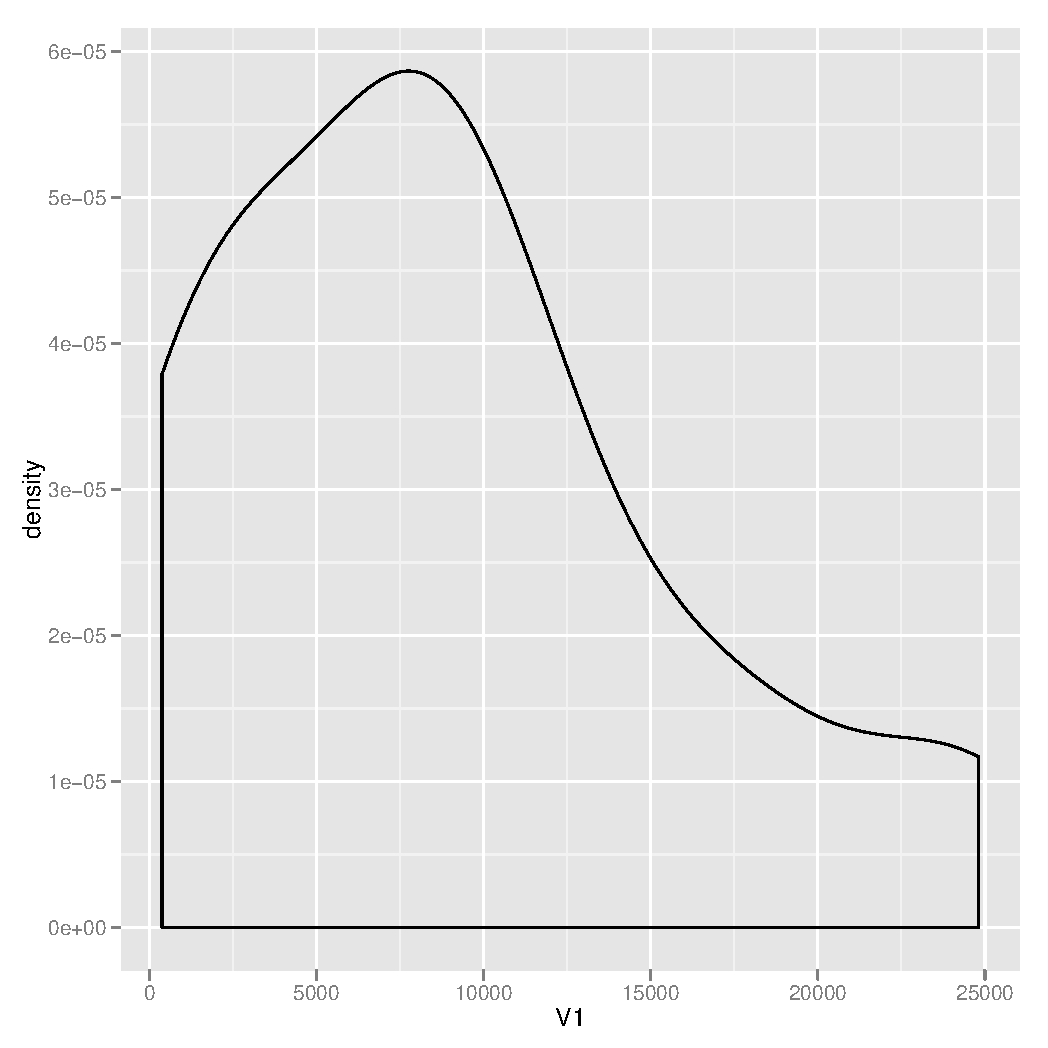
\includegraphics[width=\textwidth]{plot1.pdf}
\caption{plot1.pdf}
\label{fig:plot1.pdf}
\end{figure}
\clearpage

\section{Second letter}
\begin{figure}[!h]
\centering
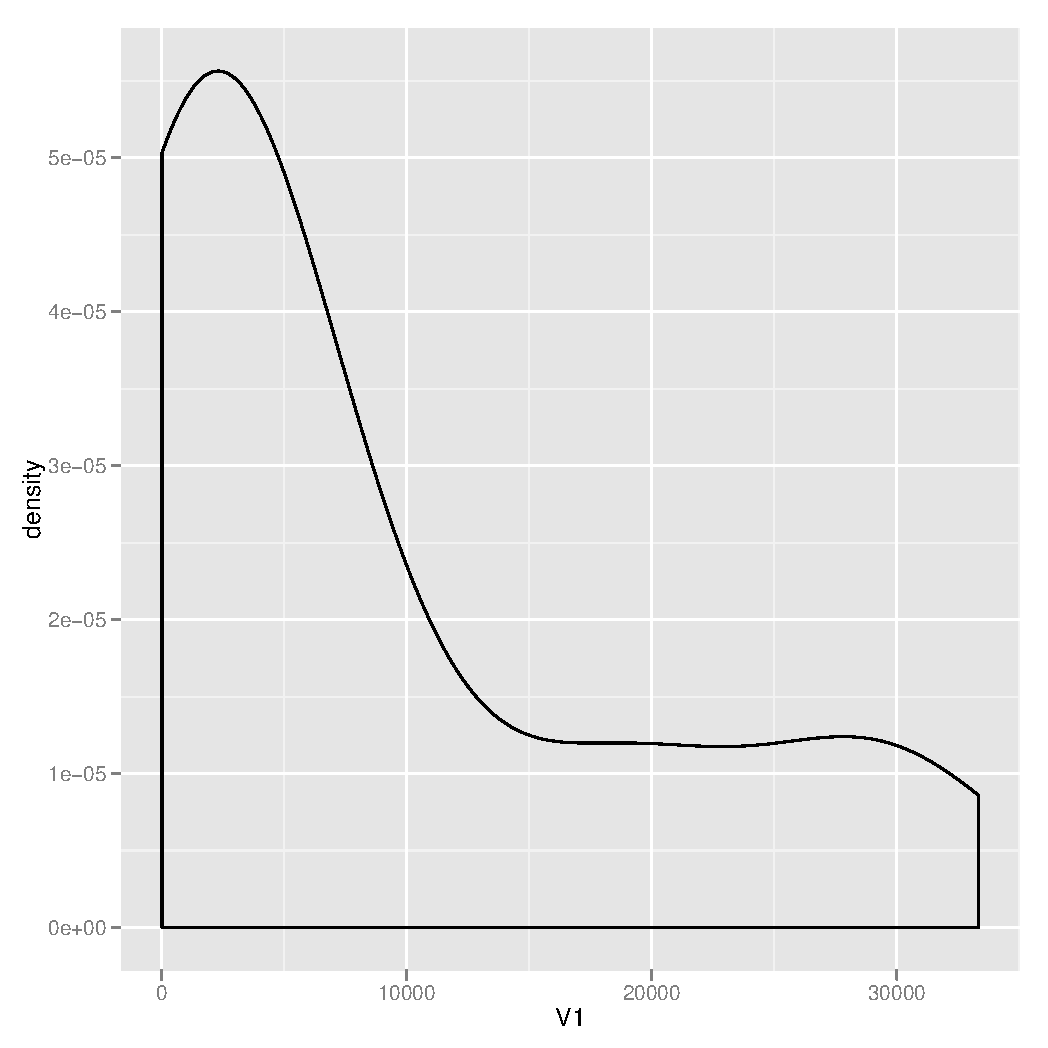
\includegraphics[width=\textwidth]{plot2.pdf}
\caption{plot2.pdf}
\label{fig:plot2.pdf}
\end{figure}
\clearpage

\section{Discussion}
We see that both the first and second letter distributions are very skewed. To make a note of this for posterity, we can write up our discovery in a text file that we store in the reports directory. Like the graphs directory, the reports directory is generated by ProjectTemplate automatically when we run create.project(). It's meant to contain the sort of written descriptions of the results of your analyses that you'd publish in a scientific paper.

\section{Conclusion}
With that report written and stored in the reports directory, we've gone through the simplest sort of analysis you might run with ProjectTemplate

\section{References}

\end{document}
